% This file was created by matlab2tikz.
%
%The latest updates can be retrieved from
%  http://www.mathworks.com/matlabcentral/fileexchange/22022-matlab2tikz-matlab2tikz
%where you can also make suggestions and rate matlab2tikz.
%
\definecolor{mycolor1}{rgb}{0.00000,0.44700,0.74100}%
\definecolor{mycolor2}{rgb}{0.85000,0.32500,0.09800}%
\definecolor{mycolor3}{rgb}{0.92900,0.69400,0.12500}%
\definecolor{mycolor4}{rgb}{0.49400,0.18400,0.55600}%
\definecolor{mycolor5}{rgb}{0.46600,0.67400,0.18800}%
%
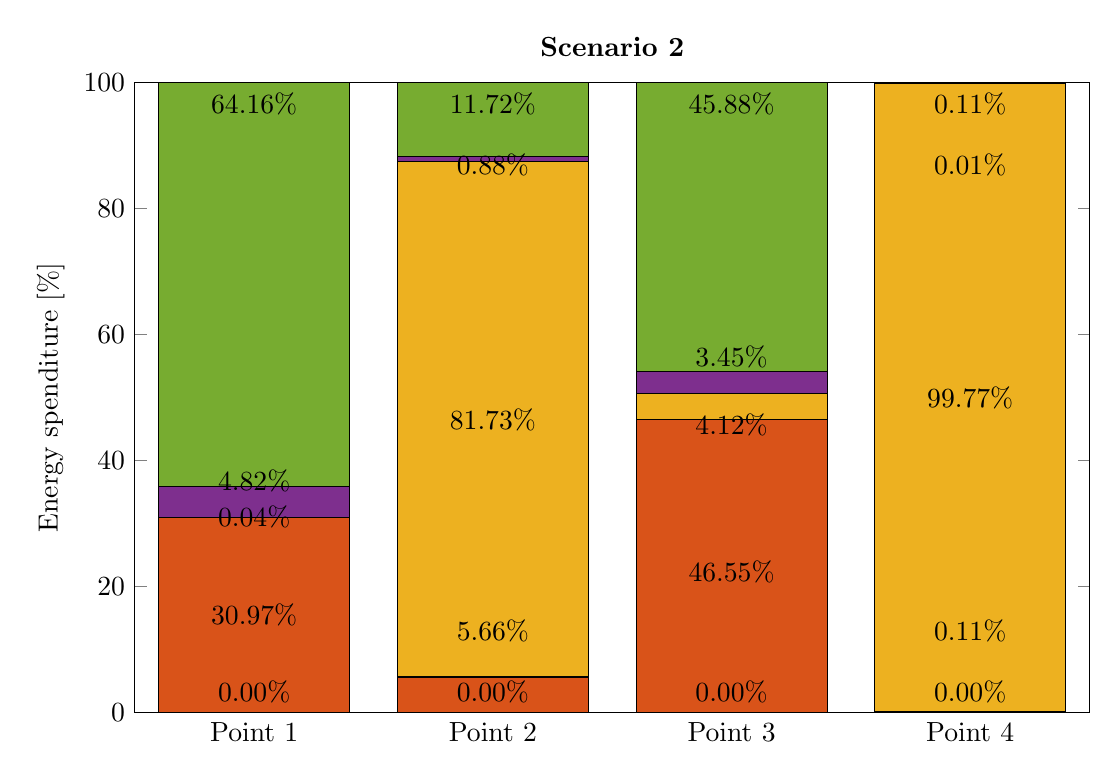
\begin{tikzpicture}

\begin{axis}[%
width=\textwidth,
height=0.66\textwidth,
at={(0.758in,0.481in)},
scale only axis,
bar width=0.8,
xmin=0.5,
xmax=4.5,
xtick={1,2,3,4},
xticklabels={Point 1, Point 2, Point 3, Point 4},
ymin=0,
ymax=100,
ylabel={Energy spenditure [\%]},
axis background/.style={fill=white},
title style={font=\bfseries},
title={Scenario 2}
]
\addplot[ybar stacked,draw=black,fill=mycolor1,area legend] plot table[row sep=crcr] {%
1	0.000160529803543664\\
2	2.93590436120821e-05\\
3	0.000114798346354448\\
4	2.78151037336133e-07\\
};
\addplot[ybar stacked,draw=black,fill=mycolor2,area legend] plot table[row sep=crcr] {%
1	30.9670012005985\\
2	5.66350620703574\\
3	46.5473515249735\\
4	0.112782061092985\\
};
\addplot[ybar stacked,draw=black,fill=mycolor3,area legend] plot table[row sep=crcr] {%
1	0.0446900403822559\\
2	81.7329128700693\\
3	4.11761168747225\\
4	99.7678101286877\\
};
\addplot[ybar stacked,draw=black,fill=mycolor4,area legend] plot table[row sep=crcr] {%
1	4.81750664863652\\
2	0.881066223695617\\
3	3.44510355464683\\
4	0.0083473251826879\\
};
\addplot[ybar stacked,draw=black,fill=mycolor5,area legend] plot table[row sep=crcr] ;
\node[align=center, text=black]
at (axis cs:1,15.484) {30.97\%};
\node[align=center, text=black]
at (axis cs:1,30.99) {0.04\%};
\node[above, align=center, text=black]
at (axis cs:1,33.421) {4.82\%};
\node[below, align=center, text=black]
at (axis cs:1,100) {64.16\%};
\node[above, align=center, text=black]
at (axis cs:2,0) {0.00\%};
\node[align=center, text=black]
at (axis cs:2,13) {5.66\%};
\node[align=center, text=black]
at (axis cs:2,46.53) {81.73\%};
\node[align=center, text=black]
at (axis cs:2,87) {0.88\%};
\node[below, align=center, text=black]
at (axis cs:2,100) {11.72\%};
\node[above, align=center, text=black]
at (axis cs:3,0) {0.00\%};
\node[align=center, text=black]
at (axis cs:3,22.274) {46.55\%};
\node[align=center, text=black]
at (axis cs:3,45.606) {4.12\%};
\node[align=center, text=black]
at (axis cs:3,56.388) {3.45\%};
\node[below, align=center, text=black]
at (axis cs:3,100) {45.88\%};
\node[above, align=center, text=black]
at (axis cs:4,0) {0.00\%};
\node[align=center, text=black]
at (axis cs:4,13) {0.11\%};
\node[align=center, text=black]
at (axis cs:4,49.997) {99.77\%};
\node[align=center, text=black]
at (axis cs:4,87) {0.01\%};
\node[below, align=center, text=black]
at (axis cs:4,100) {0.11\%};
\end{axis}
\end{tikzpicture}%